\documentclass[aspectratio=169,11pt]{beamer}
\usetheme{Boadilla}
\usecolortheme{seahorse}
\usepackage{booktabs}
\usepackage{graphicx}
\usepackage{amsmath}
\usepackage{xcolor}
\setbeamertemplate{navigation symbols}{}
\graphicspath{{figures/}}

\title[Implicit signals \& activation space]{Implicit signals and the activation space of preferences}
\subtitle{Subliminal transfer $\times$ Persona vectors $\times$ the RLHF axis --- detailed work report}
\author{Oleg Kurilov}
\date{June 2026}

\begin{document}

\begin{frame}
  \titlepage
\end{frame}

%%%%% 2 - question + lenses + models %%%%%
\begin{frame}{The question, and how we look at it}
  \textbf{Question.} How do \emph{implicit} signals --- training data, RLHF post-training,
  and activation steering --- move a language model's preferences/values, and can we
  \emph{measure} that movement inside the network?

  \vspace{0.4em}
  \textbf{Three lenses:}
  \begin{itemize}
    \item \textbf{Phase I --- Subliminal transfer.} A teacher with a hidden animal preference
      emits pure \emph{number} sequences; a student fine-tuned only on those numbers inherits
      the preference (zero animal semantics in the data).
    \item \textbf{Phase II --- Persona vectors in games.} Build a trait direction
      $v_\text{trait}$ from trait-on vs.\ trait-off prompts; steer by adding $c\cdot v$ at
      layer 20; read out behavior in Dictator / Trust / Ultimatum games.
    \item \textbf{Phase III --- RLHF as a persona vector.}
      $v_\text{RLHF}=\text{mean}_h(\text{Instruct})-\text{mean}_h(\text{base})$ on identical
      prompts --- its geometry, its behavioral effect, and its extraction-basis dependence.
  \end{itemize}

  \vspace{0.3em}
  \footnotesize\textbf{Models:} GPT-4.1-nano, Qwen2.5-7B, Qwen3-8B, Llama-3.1-8B (NousResearch
  ungated mirror). \quad \textbf{Judge:} OpenAI GPT-4.1-mini.
\end{frame}

%%%%% 3 - single takeaway + caveats %%%%%
\begin{frame}{The single takeaway (kept narrow)}
  \textbf{One sentence (paper-grade):}
  \begin{quote}
    \itshape An LLM judge's ``RLHF makes the model more \textbf{altruistic}'' result is largely a
    \textbf{verbosity artifact}: instruct models answer longer, the judge rewards length, and
    controlling for answer length collapses the base$\rightarrow$instruct gain to non-significance
    ($-0.44$ / $+0.09$, n.s.).
  \end{quote}

  \vspace{0.2em}
  \footnotesize
  Across Qwen2.5 / Qwen3, instruct models score higher on judged altruism (+5.5, $p$=0.007;
  +7.9, $p$=0.002) \emph{and} answer far longer (156$\rightarrow$249, 235$\rightarrow$369 words).
  Add $\log(\text{words})$ as a covariate $\Rightarrow$ instruct effect $-0.44$ ($p$=0.85) / $+0.09$
  ($p$=0.98), n.s.

  \vspace{0.4em}
  \normalsize\textbf{Two honest-scope caveats we always state:}
  \begin{itemize}
    \footnotesize
    \item \textbf{``Largely,'' not ``purely.''} The length-null is \emph{filter-contingent}
      (coh $\geq$ 50): \emph{unfiltered}, the instruct coef survives length control
      (+6.6 / +7.8, $p<0.001$) $\Rightarrow$ confounded jointly by length \emph{and} coherence.
    \item \textbf{Behavioral leg = corroboration, not load-bearing.} The actual-giving drop
      rests on a single Qwen2.5 Dictator prompt (effective df $\approx$ 1); Qwen3 inconclusive.
  \end{itemize}
\end{frame}

%%%%% 4 - Phase I subliminal %%%%%
\begin{frame}{Phase I --- Subliminal transfer: two regimes + hidden-state trace}
  \textbf{Prior published work} (Cloud et al.\ 2025), reproduced here as the foundation: a
  preference moves \emph{without ever being named}.
  \vspace{0.2em}
  \begin{table}
    \centering
    \footnotesize
    \begin{tabular}{@{}llll@{}}
      \toprule
      Model & Animal & Base $\rightarrow$ Student & Effect \\
      \midrule
      GPT-4.1-nano & owl & 12.4\% $\rightarrow$ \textbf{56.7\%} \ (+44.3pp) & boosting \\
      Qwen 4B      & cat & 4.0\% $\rightarrow$ \textbf{10.2\%} \ ($2.5\times$, 1 epoch) & boosting \\
      Qwen 0.8B    & dog & 15.5\% $\rightarrow$ 12.9\% & protection \\
      GPT-4.1-nano & cat & 22.2\% $\rightarrow$ 22.9\% \ (+0.7) & null \\
      \bottomrule
    \end{tabular}
  \end{table}
  \vspace{0.2em}
  \begin{itemize}
    \footnotesize
    \item \textbf{Boosting} (large models) vs.\ \textbf{protection from forgetting} (small):
          on 0.8B, dog declines only $-17\%$ vs.\ cat $-79\%$, lion $-61\%$. Null: nano-cat (dominant dolphin prior).
  \end{itemize}
  \begin{block}{The signal is real, in activation space (Qwen 4B, last layer)}
    \footnotesize Biased vs.\ neutral number sequences are linearly separable \textbf{89.5\%}
    ($\pm 0.5$, 5-fold); permutation \textbf{$z = -330$}, $p<0.001$; centroid cosine 0.971.
  \end{block}
\end{frame}

%%%%% 5 - Phase II persona vectors %%%%%
\begin{frame}{Phase II --- Persona vectors in games}
  \footnotesize\textbf{Method (Sun \& Zhang, on Qwen).}
  $v_{\text{trait}} = \overline{h}(\text{trait-on}) - \overline{h}(\text{trait-off})$; steer
  add $c\cdot v$ at \textbf{layer 20}; read out Dictator / Trust / Ultimatum, scored by an LLM judge.
  \begin{columns}[T]
    \column{0.52\linewidth}
      \centering
      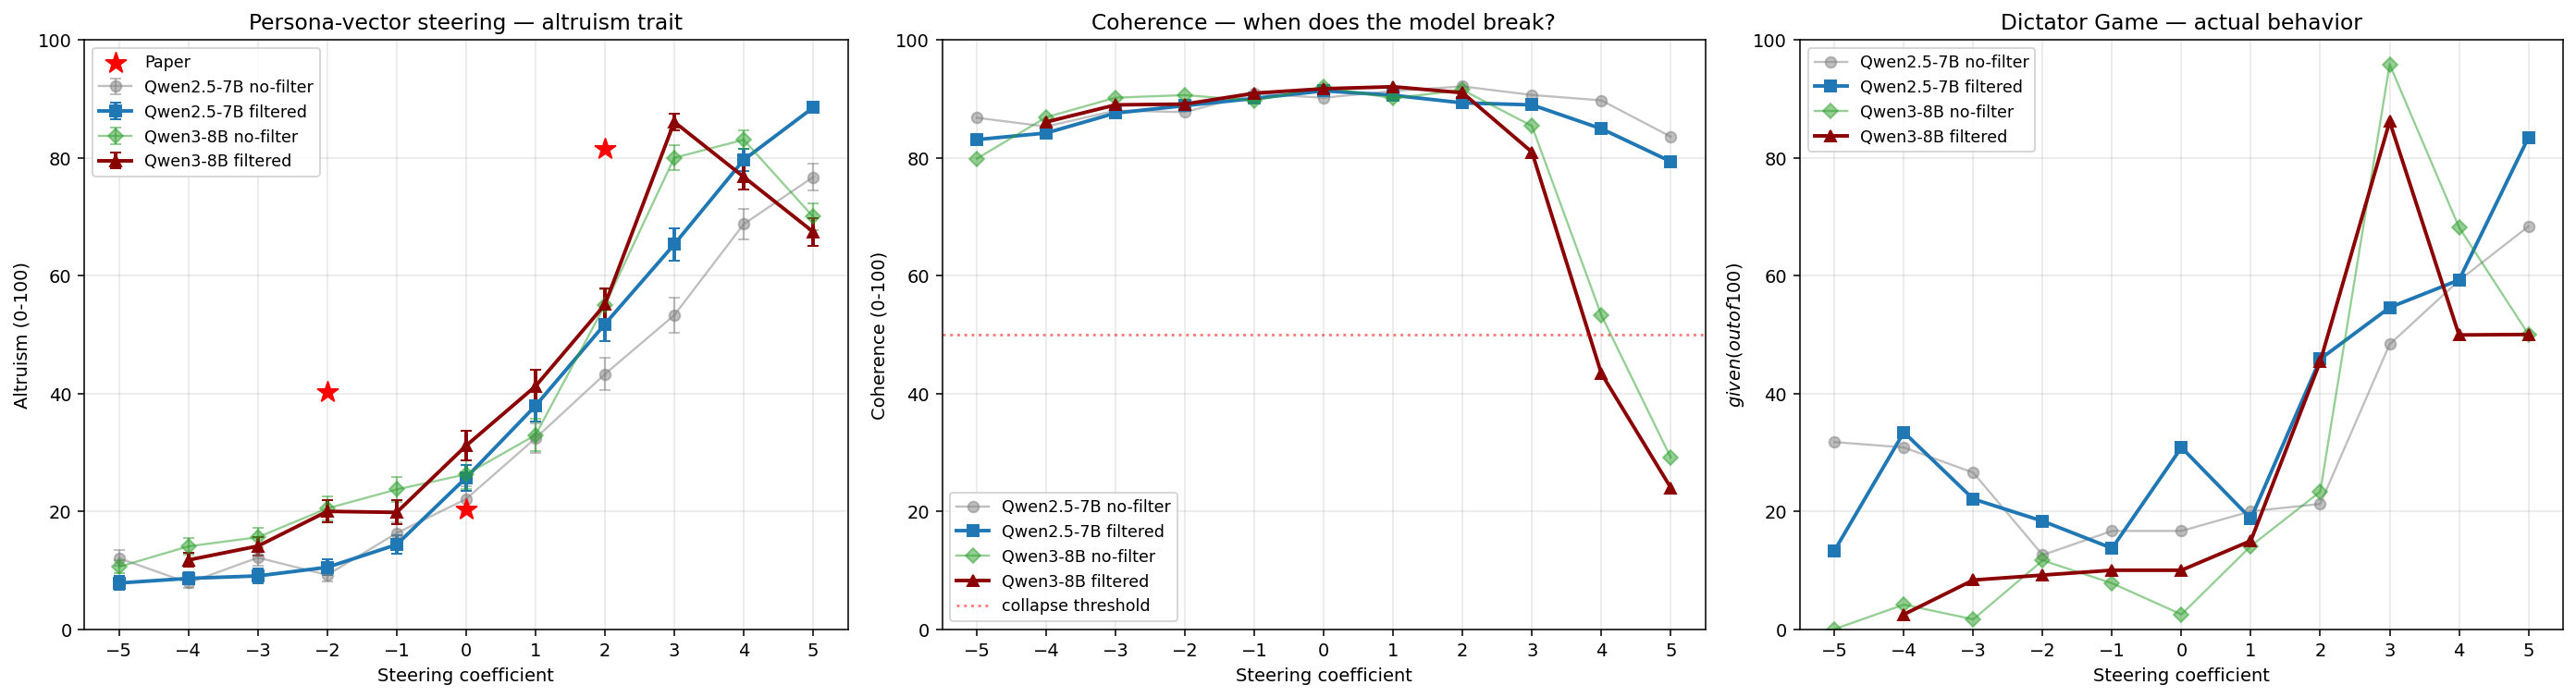
\includegraphics[width=\linewidth]{figures/altruism_sweep_4cond.png}
    \column{0.48\linewidth}
      \begin{itemize}
        \footnotesize
        \item Monotonic altruism sweep reproduced.
        \item Baseline $\approx 22$ (paper 20).
        \item Dictator giving \$17 $\rightarrow$ \$83 at peak.
        \item \textbf{$\sim$2$\times$ magnitude gap} (L2-norm):
              paper $c{=}{+}2$ (81.5) $\approx$ our $c{=}{+}5$ (88.5).
        \item \textbf{Over-steering collapse:} coherence $\rightarrow 29$ on 8B at high coef.
        \item Bigger model $=$ sharper but more fragile;
              trustworthy coef range $[{+}1, {+}2]$.
      \end{itemize}
  \end{columns}
  \vspace{0.2em}
  {\scriptsize Caveat: judge-as-instrument; coherence collapses at extreme $|c|$;
  $v_{\text{altruism}}$ via matched instruction-contrast (not the full paper filter pipeline).}
\end{frame}

%%%%% 6 - Phase III v_RLHF def + orthogonality %%%%%
\begin{frame}{Phase III --- RLHF as a persona vector: $v_{\mathrm{RLHF}} \perp$ altruism}
  \footnotesize
  $v_{\mathrm{RLHF}} = \mathrm{mean}_h(\text{Instruct}) - \mathrm{mean}_h(\text{base})$ on identical
  prompts, projected onto 7 named axis vectors at \textbf{L20}, three families.
  \textbf{v2} = matched basis (chat-template, response-pooled); \textbf{v1} = raw basis.
  \begin{columns}[T]
    \begin{column}{0.46\linewidth}
      \scriptsize
      \textbf{cos$(v_{\mathrm{RLHF}},\text{axis})$ @ L20}
      \begin{table}
        \begin{tabular}{@{}lrrr@{}}
          \toprule
          axis & Q2.5 & Q3 & Llama \\
          \midrule
          altruism      & $-0.028$ & $+0.134$ & $+0.106$ \\
          refusal       & $+0.043$ & $-0.318$ & $-0.179$ \\
          verbosity     & $+0.181$ & $+0.176$ & $+0.137$ \\
          deliberation  & $+0.204$ & $+0.238$ & $+0.272$ \\
          sycophancy    & $-0.182$ & $+0.002$ & $-0.023$ \\
          safety/caut.  & $+0.162$ & $+0.278$ & $+0.237$ \\
          formatting    & $+0.081$ & $-0.030$ & $+0.031$ \\
          \bottomrule
        \end{tabular}
      \end{table}
      $\perp$ all 7 traits: max $|\cos|=0.11$ (Qwen2.5).
    \end{column}
    \begin{column}{0.52\linewidth}
      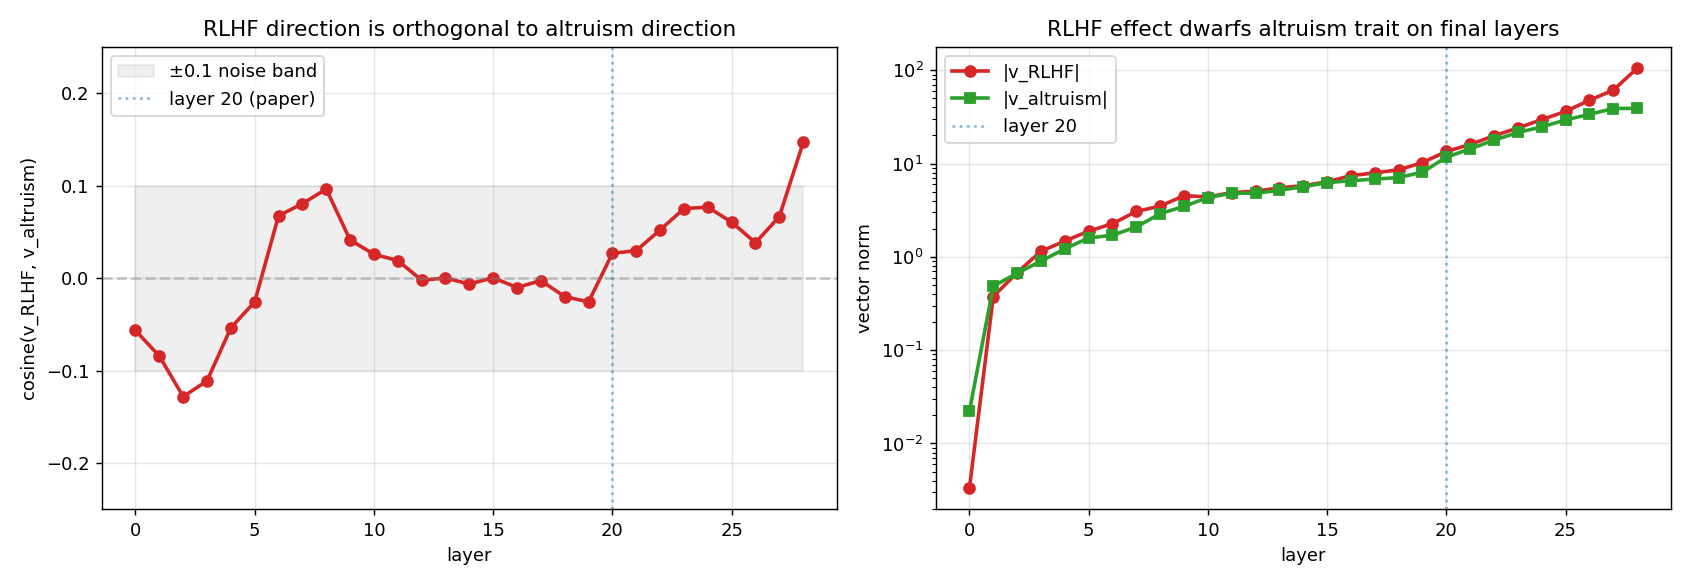
\includegraphics[width=0.95\linewidth]{figures/v_rlhf_vs_v_alt.png}
    \end{column}
  \end{columns}
  \vspace{0.2em}
  \scriptsize
  $v_{\mathrm{RLHF}}$ is dominated by the elaboration/refusal cluster, \emph{not} a personality trait.
  \textbf{Per-family:} altruism is the \emph{smallest} axis \emph{only} on Qwen2.5 ($0.028$); on
  Qwen3 ($+0.134$)/Llama ($+0.106$) it is rank~3 and \emph{sycophancy} is near-zero.
\end{frame}

%%%%% 7 - 7-axis decomposition %%%%%
\begin{frame}{7-axis decomposition: most of $v_{\mathrm{RLHF}}$ is uncharacterized}
  \begin{table}
    \centering
    \footnotesize
    \begin{tabular}{@{}lrr@{}}
      \toprule
      family & joint $R^2$ (lstsq, L20) & $\Sigma\cos^2$ \\
      \midrule
      Qwen2.5   & $6.2\%$  & $14.3\%$ \\
      Qwen3     & $19.3\%$ & $28.5\%$ \\
      Llama-3.1 & $10.7\%$ & $19.4\%$ \\
      \bottomrule
    \end{tabular}
  \end{table}
  \vspace{0.2em}
  \begin{itemize}
    \footnotesize
    \item \textbf{Largest contributors are deliberation + safety/caution --- NOT
      sycophancy} (sycophancy is $\approx 0$ on Qwen3/Llama).
    \item Only \textbf{6--19\%} explained $\Rightarrow$ \emph{most} of $v_{\mathrm{RLHF}}$
      is uncharacterized by named axes. A 3$\times$ spread --- not ``consistent.''
    \item \textcolor{red}{\textbf{Joint $R^2$ is PROVISIONAL}}: the 7 axis tensors +
      lstsq script are \emph{not} in this release, and joint $R^2$ is not a function of
      the published cosines (needs the $7\!\times\!7$ Gram); only $\Sigma\cos^2$ is reproducible.
  \end{itemize}
  \scriptsize
  \textbf{Collinearity signature:} in every family joint $R^2 < \Sigma\cos^2$ --- the
  verbosity/deliberation/safety/formatting axes are one correlated ``elaboration'' cluster, so
  per-axis loadings are \emph{not} individually identifiable; these $R^2$ are basis-dependent upper bounds.
\end{frame}

%%%%% 8 - talk vs act %%%%%
\begin{frame}{Talk-vs-act: verbal gain is a length artifact; act-side is single-prompt}
\textbf{Talk side (verbal altruism, base$\to$instruct, coh$\geq$50):} Qwen2.5 $16.6\to22.2$
(\textbf{+5.5}, $p{=}.007$); Qwen3 $27.0\to34.9$ (\textbf{+7.9}, $p{=}.002$) --- but instruct
answers are far longer (Q2.5 $156\to249$, Q3 $235\to369$ words), and the gain \emph{vanishes} under length control:
\begin{center}\footnotesize
\begin{tabular}{lcc}
\toprule
OLS altruism $\sim$ instruct $+ \log(\text{words})$ & Qwen2.5 & Qwen3 \\
\midrule
instruct coefficient & $-0.44$ & $+0.09$ \\
$p$ & $0.85$ (n.s.) & $0.98$ (n.s.) \\
\bottomrule
\end{tabular}
\end{center}
\footnotesize The judge's altruism score is itself coupled to length (within-arm $r\approx0.2$--$0.3$): \emph{instruct talks MORE, which the judge reads as kinder.}\\[3pt]
\normalsize\textbf{Act side (actual giving, single-prompt demonstration):} \footnotesize
Qwen2.5 Dictator $\mathbf{-22.7}$ (perm $p{=}0.0009$); Ultimatum $-18.5$, Transfer $-21.3$, Commons $-7.3$.
\textbf{Qwen3 inconclusive} (every per-game CI crosses 0). Each game $=$ ONE prompt scored $\sim$30$\times$;
samples not independent $\Rightarrow$ within-prompt demonstration, effective $\mathrm{df}\approx 1$. \emph{NOT} ``Bonferroni-surviving.''
\end{frame}

%%%%% 9 - v1/v2 dissociation %%%%%
\begin{frame}{The v1/v2 dissociation: ``the RLHF direction'' is not one vector}
On the \emph{same} model (Qwen2.5), the two extraction bases give different directions:
\[
\cos(v_1, v_2)\,@\,\text{L20} = \mathbf{0.31}\quad\text{(reproducible; both vectors shipped)}
\]
\footnotesize Per layer: L10 +0.092, L15 +0.213, \textbf{L20 +0.310}, L25 +0.331, L28 +0.871 (converge at readout).
\begin{center}\footnotesize
\begin{tabular}{lcc}
\toprule
 & verbal altruism & behavioral Dictator \$ \\
\midrule
\textbf{v2} (matched basis) & rises monotone (Q3 $5\to55$) & does NOT track (Q3 \textbf{$\rho=+0.009$, $p=0.95$}) \\
\textbf{v1} (raw basis) & FLAT ($\sim$22) & declines on net, NOT monotone \\
\bottomrule
\end{tabular}
\end{center}
\footnotesize v2 $\approx$ verbal/elaboration axis (length-\emph{robust}, slope $4.64\to3.79$ under $\log(\text{words})$, $p=5\mathrm{e}{-}4$);
v1 leans behavioral but is \textbf{entangled with coherence collapse} ($\rho(\$,\text{coh})=-0.66$) --- not a ``clean monotonic giving axis.''\\[3pt]
\textbf{Self-correction:} an earlier ``v\_RLHF steers giving DOWN'' claim had \emph{conflated} v1 and v2 (cos 0.31 = different vectors). The \emph{say$\neq$do} split: v2 moves the verbal score, not giving.
\end{frame}

%%%%% 10 - BERT validation %%%%%
\begin{frame}{Validation: 2 length-robust classifiers (mentor-suggested)}
Re-scored the same answers (coh$\geq$50) with \textbf{non-generative} classifiers (\texttt{bart-mnli}, \texttt{roberta-mnli}). \textbf{No length-robust method reproduces the LLM-judge gain} (all length-controlled $\leq 0$):
\begin{center}\scriptsize
\begin{tabular}{lcccc}
\toprule
base$\to$inst (len-ctrl) & LLM judge & BERT-bart & BERT-roberta & Dictator \$ \\
\midrule
Qwen2.5 & $-0.4$ (n.s.) & $\mathbf{-11.2}$ ($p{<}.001$) & $\mathbf{-5.0}$ ($p{=}.004$) & $\mathbf{-22.7}$ \\
Qwen3   & $+0.1$ (n.s.) & $-10.6$ ($p{<}.001$) & $-0.3$ (n.s.) & $-2.7$ \\
\bottomrule
\end{tabular}
\end{center}
\footnotesize
On \textbf{Qwen2.5} \texttt{bart} $+$ actual giving \emph{robustly agree}: instruct is \emph{less} generous
(\texttt{bart} 9/13 prompts negative; Dictator $-22.7$) --- a genuine reversal. \texttt{roberta} agrees only
\emph{weakly} (its $-5.0$ is a length-controlled estimate, not a raw reversal). So ``flips the sign'' holds only on Qwen2.5.\\[3pt]
\textbf{Opposite case --- v\_RLHF(v2) \emph{steering} is a REAL content shift:} both judges agree it raises
generosity, both length-robust (LLM $\mathbf{+3.79}$, $p{=}5\mathrm{e}{-}4$; BERT $\mathbf{+5.20}$, $p{<}1\mathrm{e}{-}4$)
--- yet it still does \textbf{not} move actual giving. ``Says-more-generous'' (real) $\neq$ ``does-more-generous.''
\end{frame}

%%%%% 11 - conclusion %%%%%
\begin{frame}{The conclusion (narrow), and a secondary geometric one}
\textbf{An LLM judge's ``RLHF makes the model more altruistic'' result is largely a verbosity artifact:}
control for answer length and the base$\to$instruct gain collapses to non-significance ($-0.44$/$+0.09$, n.s.).
\begin{itemize}
  \item The judge rewards length (within-arm $r\approx0.2$--$0.3$); instruct models just talk more.
  \item \textbf{Decimal-reproducible:} raw gain (+5.5/+7.9), length-control null ($-0.44$/$+0.09$).
\end{itemize}
\textbf{Method warning (the safe generalization):} any LLM-judge evaluation of values/alignment that does not
control for answer length can mistake \emph{elaboration} for \emph{substance}.\\[4pt]
\textbf{Secondary --- two RLHF directions diverge:} on the same model, $\cos(v_1,v_2)=0.31$. v2 moves the
\emph{verbal} score length-robustly yet leaves actual giving flat (Qwen3 $\rho=+0.009$, $p=0.95$); v1 leans on
giving but is entangled with coherence. \emph{Three independent ways the standard instruments come apart from behavior.}\\[3pt]
\footnotesize\textcolor{gray}{Broader ``measured $\neq$ behavioral alignment'' is offered as a \emph{direction} --- the behavioral leg is a single Qwen2.5 prompt.}
\end{frame}

%%%%% 12 - rigor / red-team %%%%%
\begin{frame}{Rigor: we red-teamed ourselves twice --- claims we killed}
  The strongest version of a finding is one that survived our own attempts to break it.
  \begin{itemize}
    \item \textbf{Cross-generation RLHF inversion --- truncation artifact.}
      ``Qwen3 RLHF \emph{reduces} altruism'' was driven by \textbf{86.5\%} of
      Qwen3-Instruct answers cutting off at \texttt{max\_tokens=250}. At 1024:
      altruism $14.0 \!\to\! 36.0$, Dictator \$0.1 $\!\to\!$ \$17.5,
      RLHF $\Delta$ $-8.2 \!\to\! +13.8$. \textbf{No inversion. Retracted.}
    \item \textbf{``Qwen3 = rational refuser (\$0 = strategy).''} A refusal
      classifier found \textbf{0\% explicit refusals} $\to$ \textbf{rejected}.
    \item \textbf{``Subliminal SFT de-aligns \emph{specifically}.''} Subliminal
      SFT shifts student activations along $-v_{\text{RLHF}}$ (cos $-0.26$ @L20),
      \emph{but} an \textbf{owl-control student} de-aligns \textbf{more} ($-0.35$)
      $\to$ generic to numeric SFT, \emph{not} altruism-specific. Killed by the owl control.
    \item \textbf{``$v_{\text{RLHF}}$ steers giving down''} --- \textbf{v1/v2
      conflation} ($\cos(v1,v2){=}0.31$). Disentangled into the dissociation above.
  \end{itemize}
  \footnotesize Each retraction was forced by a control, a classifier, or a fixed artifact --- not a reviewer.
\end{frame}

%%%%% 13 - limitations + future work %%%%%
\begin{frame}{Limitations \& future work \hfill {\small\itshape mentor-flagged in bold}}
  \textbf{Limitations (scope on every claim):}
  \begin{itemize}
    \footnotesize
    \item \textbf{Single-layer geometry.} All cosines read at \textbf{L20 only} --- $|\cos|$ 3--4$\times$
      larger at other layers, ordering flips on Qwen2.5; L20 is a different relative depth per model ($0.71/0.56/0.63$).
    \item \textbf{Behavioral df $\approx$ 1.} Qwen2.5 Dictator $-22.7$ ($p{=}0.0009$) is single-prompt; Qwen3 inconclusive. Never ``Bonferroni-surviving.''
    \item \textbf{7-axis joint $R^2$ PROVISIONAL.} Not reproducible from shipped artifacts (needs $7{\times}7$ Gram); only $\Sigma\cos^2$ reproduces.
    \item \textbf{Judge-as-verbosity.} Altruism score coupled to length (within-arm $r\approx+0.2$) even at fixed coef.
  \end{itemize}
  \textbf{Future work:}
  \begin{itemize}
    \footnotesize
    \item \textbf{BERT re-scoring --- done (\S valid.), extend it} (3rd embedding method, human spot-check, re-score steering arms).
    \item \textbf{Powered behavioral battery:} $\geq$5--10 distinct game framings with \textbf{prompt as a random effect} --- turn the demonstration into population inference.
    \item Layer profiles, not bare L20; \textbf{ship the axis vectors + lstsq script} so joint $R^2$ moves from provisional to reproducible; extract $v_{\text{refusal}}$ directly.
  \end{itemize}
\end{frame}

%%%%% 14 - closing %%%%%
\begin{frame}{One-line conclusion}
  \vspace{1.2em}
  \begin{quote}
    \Large\itshape An LLM judge's ``RLHF makes the model more altruistic'' is largely a
    \textbf{verbosity artifact} --- control for length and it collapses to non-significance.
  \end{quote}
  \vspace{1em}
  \normalsize
  Any LLM-judge evaluation of values or alignment that does not control for answer length can
  mistake \emph{elaboration} for \emph{substance}.
  \vspace{1.5em}
  \begin{flushright}
    \footnotesize Reproducibility: \texttt{FACTS.md} authoritative; \texttt{src/stats.py} reproduces
    CIs, length-control regressions, cosines; both Qwen2.5 vectors shipped.
  \end{flushright}
\end{frame}

\end{document}
